\documentclass[aspectratio=169, 8pt,t]{beamer}
\graphicspath{{figures/}} % Setting the graphicspath

% Theme settings
\usetheme{Madrid}
\usecolortheme{default}
\setbeamertemplate{navigation symbols}{}   % removes navigation symbols such as 'next page'
\setbeamertemplate{footline}{}             % remove line with name, date, page nr. 
\setbeamercolor*{frametitle}{bg=white}     % remove background from frametitle
\usepackage{caption}
% \captionsetup[figure]{labelformat=empty}% redefines the caption setup of the figures environment in the beamer class.
\setbeamersize{text margin left=20pt,text margin right=10pt}
\usefonttheme[onlymath]{serif} % makes beamer math look like article math
\usepackage{hyperref}


%======================= page numbering =======================
\addtobeamertemplate{navigation symbols}{}{ \usebeamerfont{footline}
  \insertframenumber / \inserttotalframenumber \hspace*{2mm} \\ \vspace*{1mm} 
}


%=================================== colors ====================================
\definecolor{RoyBlue}{RGB}{22, 46, 69}
\definecolor{RoyGrey}{RGB}{64, 88, 128} 

\newcommand{\hlme}[1]{{\color{red}\bf #1}} % highlight me

\setbeamercolor{structure}{fg=RoyBlue} % itemize, enumerate, etc
\setbeamercolor{frametitle}{fg=RoyGrey}
\setbeamercolor{section in head/foot}{bg=RoyBlue}


%======================= add progress dots to headline =========================
\setbeamertemplate{headline}{%
    \begin{beamercolorbox}[ht=4mm,dp=4mm]{section in head/foot}
        \insertnavigation{\paperwidth}
    \end{beamercolorbox}%
}%
\makeatother


%======================= add section title page ================================
\AtBeginSection[]{
  \begin{frame}
  \vfill
  \centering
    \usebeamerfont{title}\insertsection\par%
  \vfill
  \end{frame}
}


%=================================== titlepage =================================
\title{An NNPDF4.0 determination of $\alpha_s$ -- status \& ideas}
\date{NNPDF collaboration meeting  \\[0.1cm] Gargnano, 26 September 2023}
\author{Roy Stegeman}
\institute{\small The University of Edinburgh}


\titlegraphic{\vspace*{6mm}
  
\includegraphics[height=1.5cm]{logos/edi_logo.png} \hspace{10mm}
  % 
\includegraphics[height=0.8cm]{logos/nnpdf_logo_official.pdf} \hspace{10mm}
  
\includegraphics[height=1.5cm]{logos/higgs_logo.jpg}
}

\defbeamertemplate{title page}{noinstitute}[1][]
{
  \vbox{}
  \vfill
  \begingroup
    \centering
    \begin{beamercolorbox}[sep=8pt,center,#1]{title}
      \usebeamerfont{title}\inserttitle\par%
      \ifx\insertsubtitle\@empty%
      \else%
        \vskip0.25em%
        {\usebeamerfont{subtitle}\usebeamercolor[fg]{subtitle}\insertsubtitle\par}%
      \fi%     
    \end{beamercolorbox}%
    \vskip2em\par
    \begin{beamercolorbox}[sep=0pt,center,#1]{author}
      \usebeamerfont{author}\insertauthor
    \end{beamercolorbox}
  \begin{beamercolorbox}[sep=0pt,center,#1]{author}
    \usebeamerfont{institute}\insertinstitute
  \end{beamercolorbox}
  \vspace*{8pt}
  \vspace*{16pt}
    \begin{beamercolorbox}[sep=0pt,center,#1]{date}
      \usebeamerfont{date}\insertdate
    \end{beamercolorbox}\vskip0.5em
    {\usebeamercolor[fg]{titlegraphic}\inserttitlegraphic\par}
  \endgroup
  \vfill
}

\makeatletter
\setbeamertemplate{title page}[noinstitute][colsep=-4bp,rounded=true,shadow=\beamer@themerounded@shadow]
\makeatother


\begin{document}
{
\setbeamertemplate{headline}{} % remove headline from titlepage
\begin{frame}
  \titlepage
\end{frame}
}

\setbeamertemplate{enumerate items}[default]

\pgfdeclarelayer{bg}    % declare background layer
\pgfsetlayers{bg,main}  % set the order of the layers (main is the standard layer)


% SLIDES =======================================================================


\begin{frame}{Three different methodologies}
  \begin{itemize}
    \item Correlated replica method
    \item Theory covariance method based on \textcolor{gray}{[Ball \& Pearson (2021); 2105.05114]}
    \item SIMUnet \textcolor{gray}{[Iranipour \& Ubiali (2022); 2201.07240]}
  \end{itemize}
\end{frame}


\begin{frame}{Correlated replica method -- 1802.03398}
  Determining $\alpha_s$ with a fixed input PDF results in underestimated uncertainty
  \begin{figure}
    \centering
    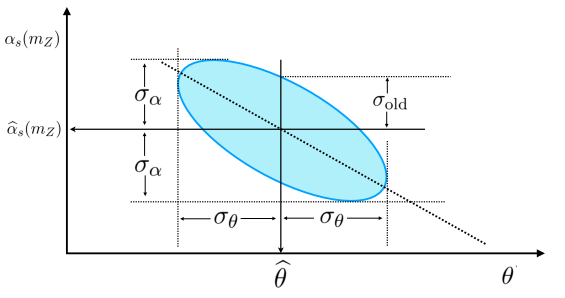
\includegraphics[width=0.7\textwidth]{figures/alphaspdfcorplot.png}
  \end{figure}
\end{frame}


\begin{frame}{Correlated replica method -- 1802.03398}
  \begin{columns}
    \column{0.5\textwidth}
    1. Produce fits to a data replica, $D^k$ at different values of $\alpha_s$, such that we can determine $\alpha_s^{(k)}=\operatorname{argmin}\left[\chi^{2(k)}\left(\alpha_s\right)\right]$ \\\vspace*{1em}
    2. Perform quadratic fit to $\chi^2$ profiles \\
    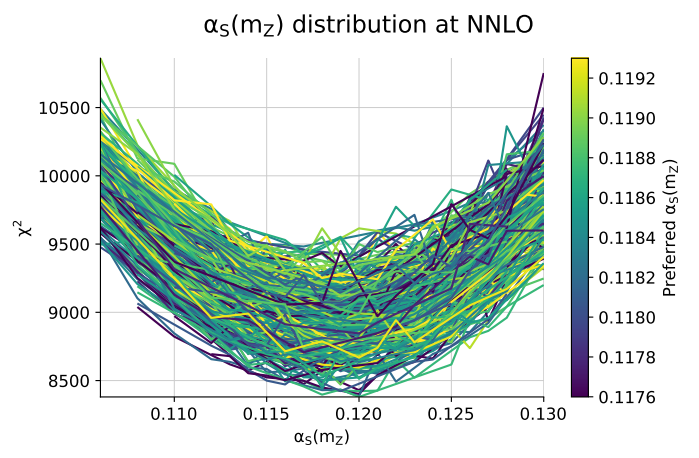
\includegraphics[width=0.9\textwidth]{figures/parabolaplotnnpdf31.png}
    \column{0.5\textwidth}
    3. Analyze the resulting probability distribution \\
    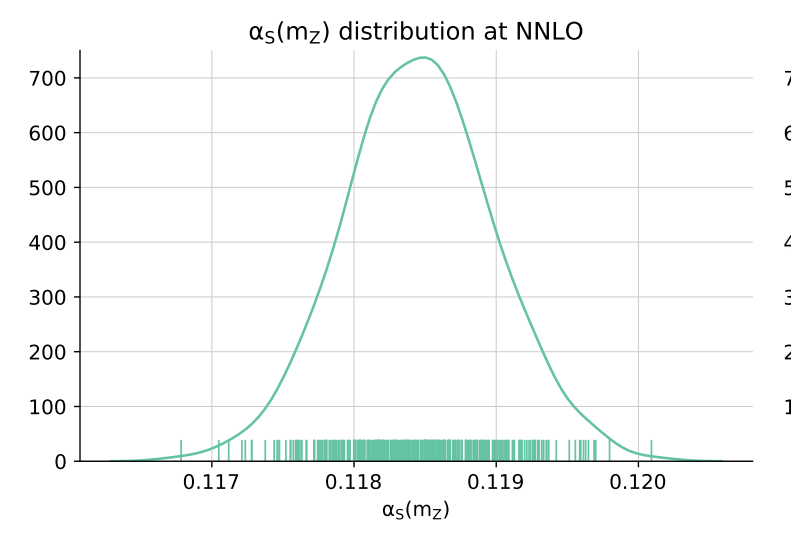
\includegraphics[width=0.9\textwidth]{figures/alphasnnpdf31result.png}
  \end{columns}
\end{frame}


\begin{frame}{Correlated replica method -- 1802.03398}
  NNPDF3.1 (arXiv:1802.03398): 0.1185 ± 0.0005

  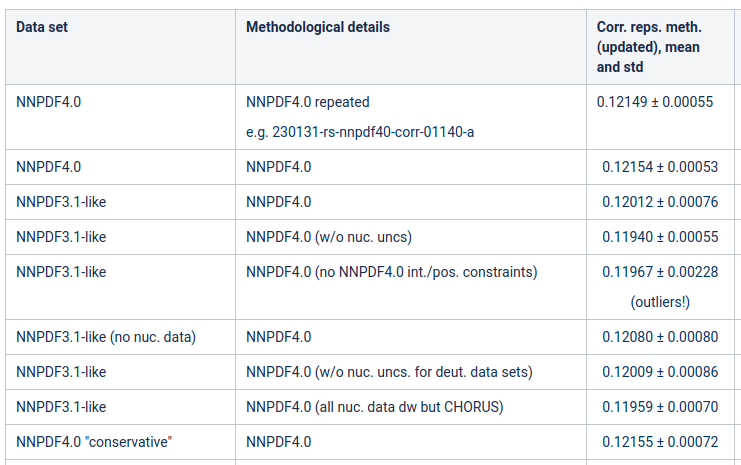
\includegraphics[width=0.5\textwidth]{figures/alphasresultstablecut.png}

  \begin{itemize}
    \item Large value of $\alpha_s$ for NNPDF4.0 compared to world average
    \item $\sim$2$\sigma$ disagreement between NNPDF3.1-like and NNPDF4.0 datasets
    \item What is the impact of MHOU?
  \end{itemize}
\end{frame}


\begin{frame}{Theory covariance method -- 2105.05114}
  $$
    P(T \mid D) \propto \exp \left(-\frac{1}{2}(T-D)^T(C+S)^{-1}(T-D)\right), \, S=\beta\beta^T \, \text{\textcolor{gray}{[Ball, Nocera, Pearson (2019); 1812.09074]}}
  $$

  Introduce a nuisance parameter $\lambda$, to model theory uncertainty as correlated shift ($T\rightarrow T+\lambda\beta$) in the theory prediction:
  $$
    P(T \mid D \lambda) \propto \exp \left(-\frac{1}{2}(T+\lambda \beta-D)^T C^{-1}(T+\lambda \beta-D)\right)
  $$

  We can marginalize over $\lambda$ to recover $P(T\mid D)$:
  $$ 
    P(T \mid D)=\int d \lambda P(T \mid D \lambda) P(\lambda)
  $$
  Which is a Gaussian integral for the choice $P(\lambda)=\exp\left(-\frac{1}{2}\lambda^2\right)$, reproducing the result on top of the slide:
  $$
    P(T \mid D) \propto \int d \lambda \exp \left(-\frac{1}{2} Z^{-1}(\lambda-\bar{\lambda})^2-\frac{1}{2} \chi^2\right) \propto \exp \left(-\frac{1}{2} \chi^2\right)
  $$

  With $Z=\left(1+\beta^T C^{-1} \beta\right)^{-1}=1-\beta^T(C+S)^{-1} \beta$ independent of $T$ and $D$, \\ and $\bar{\lambda}(T, D)=Z \beta^T C^{-1}(D-T)=\beta^T(C+S)^{-1}(D-T)$. 

\end{frame}

\begin{frame}{Theory covariance method -- 2105.05114}
  Previously we recovered the known result
  $$
    P(T \mid D) \propto \int d \lambda \exp \left(-\frac{1}{2} Z^{-1}(\lambda-\bar{\lambda})^2-\frac{1}{2} \chi^2\right) \propto \exp \left(-\frac{1}{2} \chi^2\right).
  $$

  However, we can also calculate the posterior of the nuisance parameter
  \begin{equation*}
    P(\lambda \mid T D)=\frac{P(T \mid D \lambda) P(\lambda)}{P(T \mid D)} \propto \exp \left(-\frac{1}{2} Z^{-1}(\lambda-\bar{\lambda}(T, D))^2\right)
  \end{equation*}
  where the expected value is given by $\bar{\lambda}$ and the uncertainty by $Z$.
  \vspace*{1em}

  Same idea can, with some work, be extended to the scenario of a PDF fit. This has been done by Richard and Rosalyn in their paper.

  \vspace*{1em}
  Theory covariance method (TCM) requires only a single fit!
\end{frame}


\begin{frame}{Compare CRM and TCM}
  \vspace*{-1em}
  \url{https://www.wiki.ed.ac.uk/display/nnpdfwiki/Correlated+replica+method}

  NNPDF3.1 (arXiv:1802.03398): 0.1185 ± 0.0005

  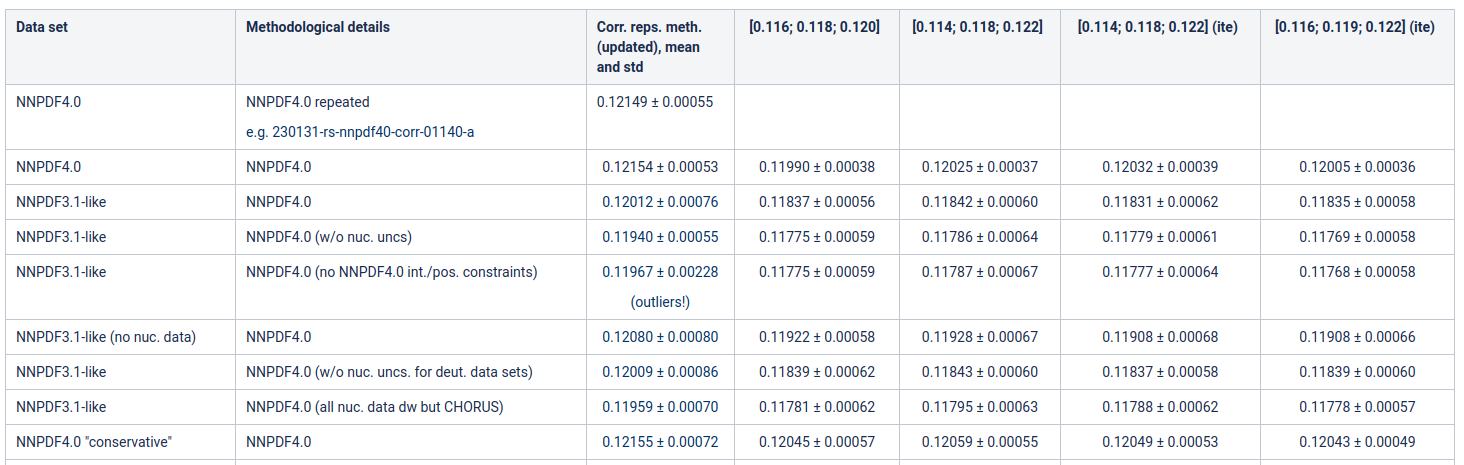
\includegraphics[width=1.0\textwidth]{figures/alphasresultstable.png}
  
  \begin{itemize}
    \item Consistent shift of $\sim$0.0017 between CRM and TCM
    \item TCM stable upon changes to prior
  \end{itemize}

\end{frame}


\begin{frame}{Compare CRM and TCM}

  CRM and TCM disagree, but there exist differences between the methodologies. We have attempted to understand these differences and obtain the same (though not necessarily the correct) result by trying the following:
  \begin{itemize}
    \item t0 PDF varies between $\alpha_s$ in CRM $\rightarrow$ fix t0 PDF at all values of $\alpha_s$
    \item Non-Gaussianity of CRM $\rightarrow$ minimal effect in most cases but keep in mind
    \item Theory covariance deweights data with large theory uncertainty in TCM $\rightarrow$ include theory covmat in CRM
    \item TCM assumes fitting and sampling covmat are the same $\rightarrow$ use the t0 covmat for both sampling and fitting in CRM and TCM
  \end{itemize}

  \vspace*{1em}

  However, this results in shifts that differ per dataset and the pattern of the consistent shifts is lost

  \vspace*{1em}

  To be tested: what is the impact of expanding chi2 beyond quadratic in the nuisance parameter?

\end{frame}

\begin{frame}{SIMUnet -- the basic idea}
  \begin{figure}
    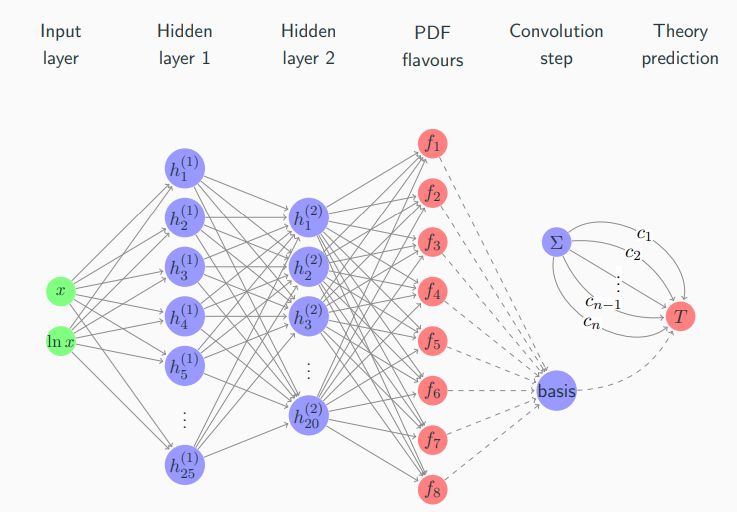
\includegraphics[width=0.5\textwidth]{figures/simunet_schematic.png}
  \end{figure}
  Can we use this to determine $\alpha_s$ by interpolating between FKTables?\\
  Note that this involves loading many different theories and is thus very memory-expensive
\end{frame}


\begin{frame}[t]{SIMUnet}
  NNPDF3.1-like dataset w/o nucl. uncertainties\\\vspace*{0.5em}

  High training-validation losses\\
  % and non-homogenous distribution of $\alpha_s$ in the tr-vl plot \\
  $\rightarrow$ problem with optimization {\color{red} (possible to solve by careful tuning and initial freezing)}\\\vspace*{0.5em}

  Two peaks in the $\alpha_s$ distribution \\
  $\rightarrow$ peak at lower $\alpha_s$ corresponds to worse $\chi^2$ \\
  $\rightarrow$ problem with optimization \\\vspace*{0.5em}

  $\alpha_s$ depends on training fraction (and what else?) and result smaller than CRM

  \vspace*{-8mm}
  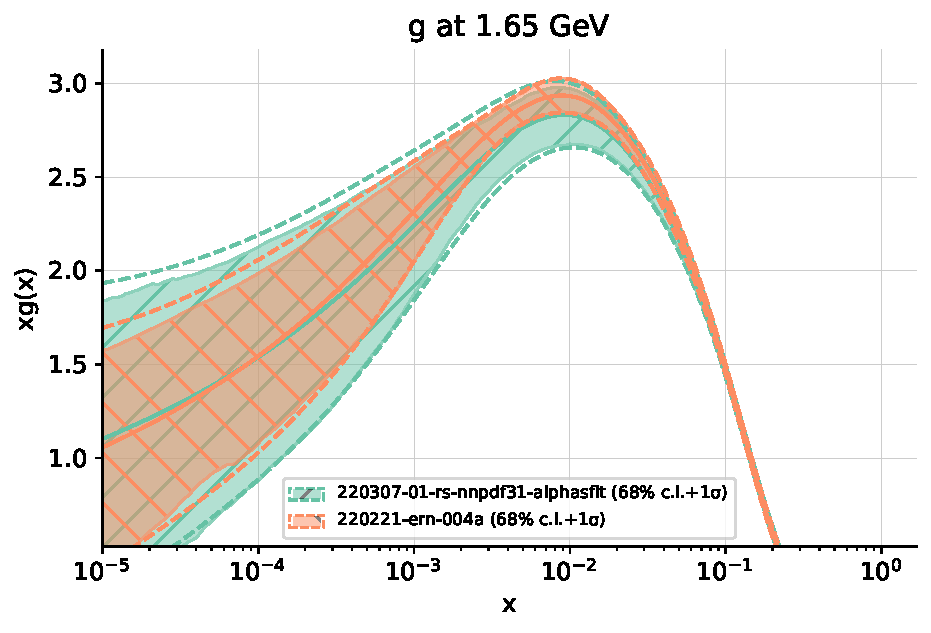
\includegraphics[width=0.32\textwidth]{PDFnormalize0_Basespecs0_PDFscalespecs0_plot_pdfs_g_prev.pdf}
  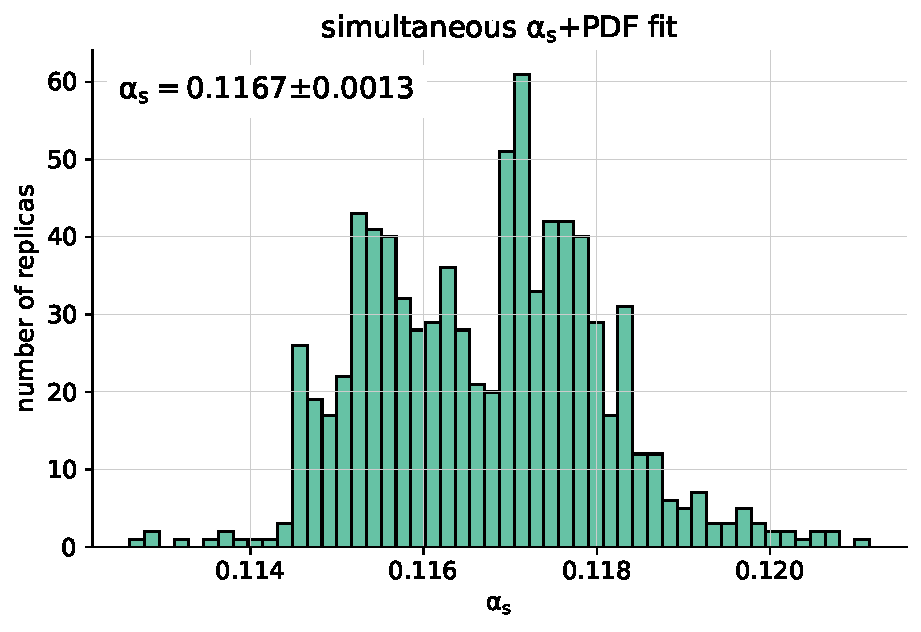
\includegraphics[width=0.32\textwidth]{alphas_hist_prev.pdf}
  % 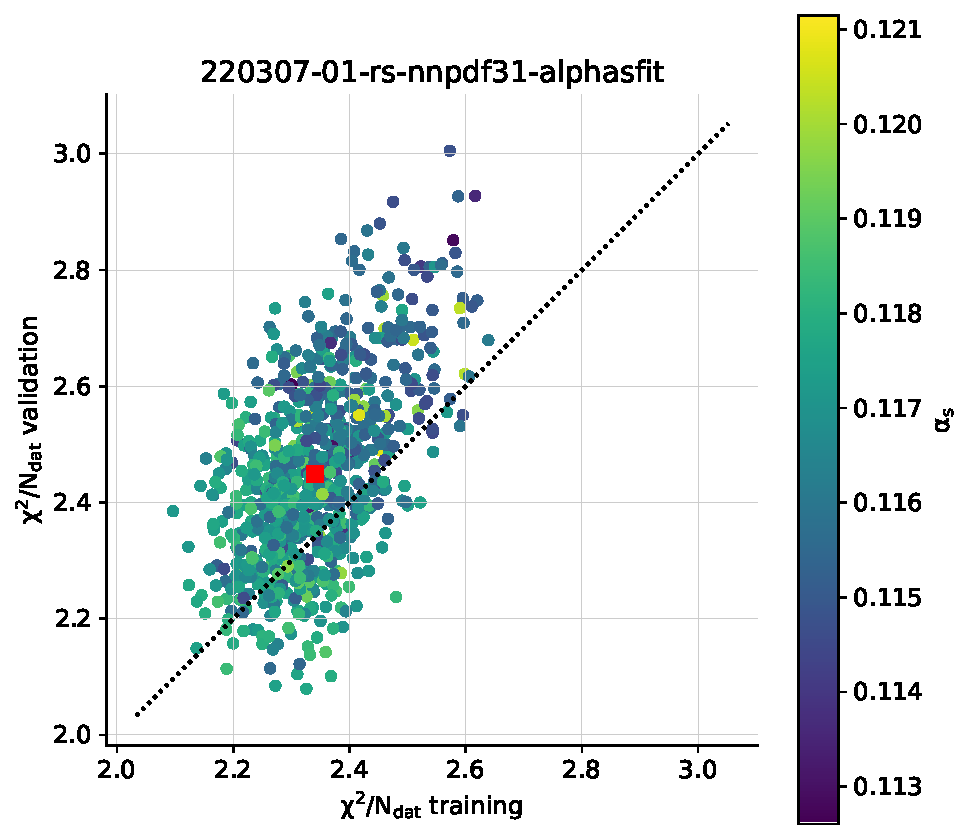
\includegraphics[width=0.32\textwidth]{plot_training_validation_prev.pdf}

  \textbf{Idea:} freeze $\alpha_s$ during the initial training to improve stability and then small learning rate

\end{frame}


\begin{frame}{SIMUnet}
  \textbf{Problem:} $\alpha_s$ doesn't stabilize and depends on initial value
  \begin{figure}
    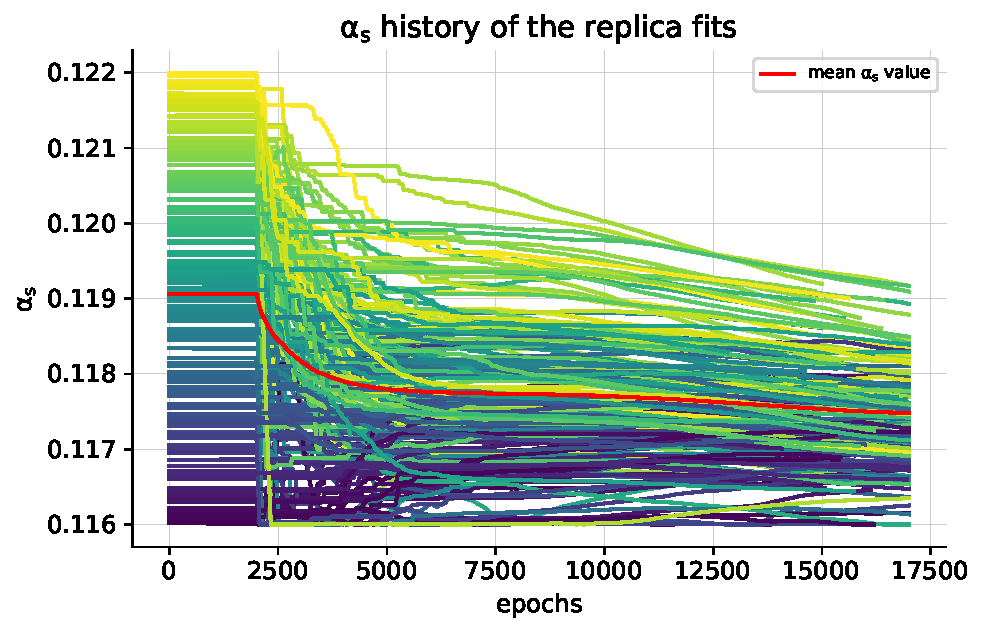
\includegraphics[width=0.52\textwidth]{figures/alphasovertime.pdf}
  \end{figure}

  % SIMUnet perhaps not suitable for $\alpha_s$ determination but can it validate the TCM and CRM in a toy-model scenario?
\end{frame}


\begin{frame}{Way forward?}
  \begin{itemize}
    \item Beyond quadratic expansion for TCM
    \item MHOU
    \item How to improve the training in SIMUnet?
    \item \ldots ?
  \end{itemize}
\end{frame}




\end{document}
